\documentclass[11pt,a4paper]{article}
\usepackage[utf8]{inputenc}
\usepackage{amsmath}
\usepackage{amsfonts}
\usepackage{amssymb}
\usepackage{graphicx}
\usepackage[font=small,skip=0pt]{caption}

\author{Silvano Garnerone}
\title{Exploratory data analysis for TISBA}
\begin{document}
\maketitle
We build descriptor vectors, labelled by dataset and region $D_{set;reg}$ containing the number of RC per bin on the genome. 
We then want to compare descriptors, and this can be done using different metrics: the Kullback-Leibner divergence, the 1-norm, the 2-norm, the cosine distance, and so on. Because of its intuitive meaning and because it provides finite results for all datasets we will stick to the cosine distance [referred to as $d(\cdot;\cdot)$]. 

\section{Noise threshold}
The value of $d(D_{set1,reg1};D_{set2,reg2})$ is affected by noise, so it is important to estimate the amount of noise to which this metric is subjected. We can also argue that the metric will depend on the amount of reads, the more reads we have the higher the accuracy of our metric estimation. To corroborate this intuition and to quantify the noise we can use XZ19-20 and XZ21-22 and XZ23-24, since they are sort of technical replicate experiments. For each of them we evaluate the distance at a given region: 
$$
d(D_{xz19,reg};D_{xz20,reg}) \;\; \forall reg \in \{A1,A2,\cdots\}
$$
and we plot it as a function of the average read-count at the given regions. 

\begin{figure}[hbtp]
\centering
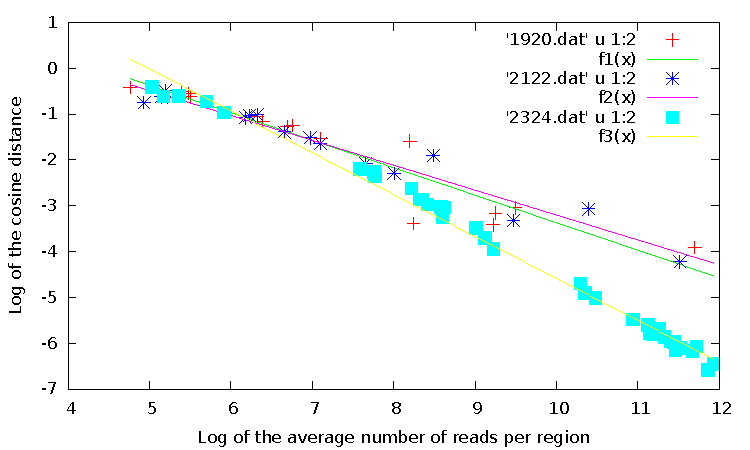
\includegraphics[scale=1]{distanceVSreads.pdf}
\caption{The log-log plot of the scaling of the distance with the average read-count. There are more data-points in XZ23-24 because typically each region has more read counts.}
\label{Fig:dist_count}
\end{figure}

As can be seen in Fig.\ref{Fig:dist_count}, XZ19-20 and XZ21-22 behaves similarly, while XZ23-24 suggests a higher degree of similarity -- for the same amount of reads -- compared to the other two datasets. This might be consistent with two interpretations: either each region in XZ23-24 is a replicate of the same heterogeneous block of cancer cells; or each region in XZ23-24 has mainly stroma cells, which are all identical to each other. The fitting curves can be used to distinguish between noise and signal in estimating the distance between two instances. Fig.\ref{Fig:filter_noise} shows the result of this filtering on XZ1920 vs XZ2122, and XZ13 vs XZ14. As can be seen, most of the points lies above the noise boundary lines, supporting the fact that most of the data provide meaningful information. A more careful analysis should provide some boundary around the solid lines.

\begin{figure}[hbtp]
\centering
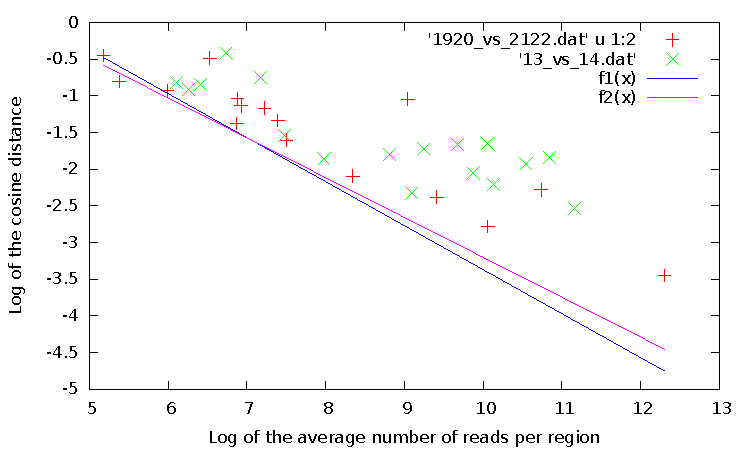
\includegraphics[scale=1]{filter_noise.pdf}
\caption{For a given pair of experiment, the distance between the local descriptor is assumed to be significant if it is above the solid lines, which represent the estimated technical noise. Regions containing less than 100 read-counts have been filtered out.}
\label{Fig:filter_noise}
\end{figure}

In Fig.\ref{fig:intra_tumor_heterog__q10_res100k} we plot the same quantities but looking at all datasets together. The noise boundary line is given by the comparison of spatially co-localized regions in XZ19+XZ20, in XZ21+22 and in XZ23+24; while all other points are related to all possible pair of regions in a given dataset.

\begin{figure}[hbtp]
\centering
\includegraphics[scale=1]{intra_tumor_heterog__q10_res100k.pdf}
\caption{Cosine distance versus number of reads.}
\label{fig:intra_tumor_heterog__q10_res100k}
\end{figure}

\section{ITH index}
We can also provide a summary of ITH with a single number. One way to do this is to consider the descriptor-vectors of  different spatial regions as instances of some high-dimensional probability distribution. The average descriptor-vector will provide the summary description obtained averaging over different spatial locations. The fluctuation of the distances between the mean vector and the vectors from each individual region is an indication of the heterogeneity of the high-dimensional probability distribution: this can define our index of ITH with possible candidates like the standard deviation or the Shannon entropy. For the moment we use the standard deviation. Fig.\ref{fig:histo_small} and Fig.\ref{fig:histo_big} show the result of this analysis for the small and large datasets that we have. The large dataset -- XZ23-24 -- has lower ITH and possible explanations are: at the resolution (related to the number of cells coming from a single region) of XZ23-24 we do not distinguish any more between different spatial locations; stroma cells are the predominant component in each region, and they all look the same. 
		
\begin{figure}[hbtp]
\centering
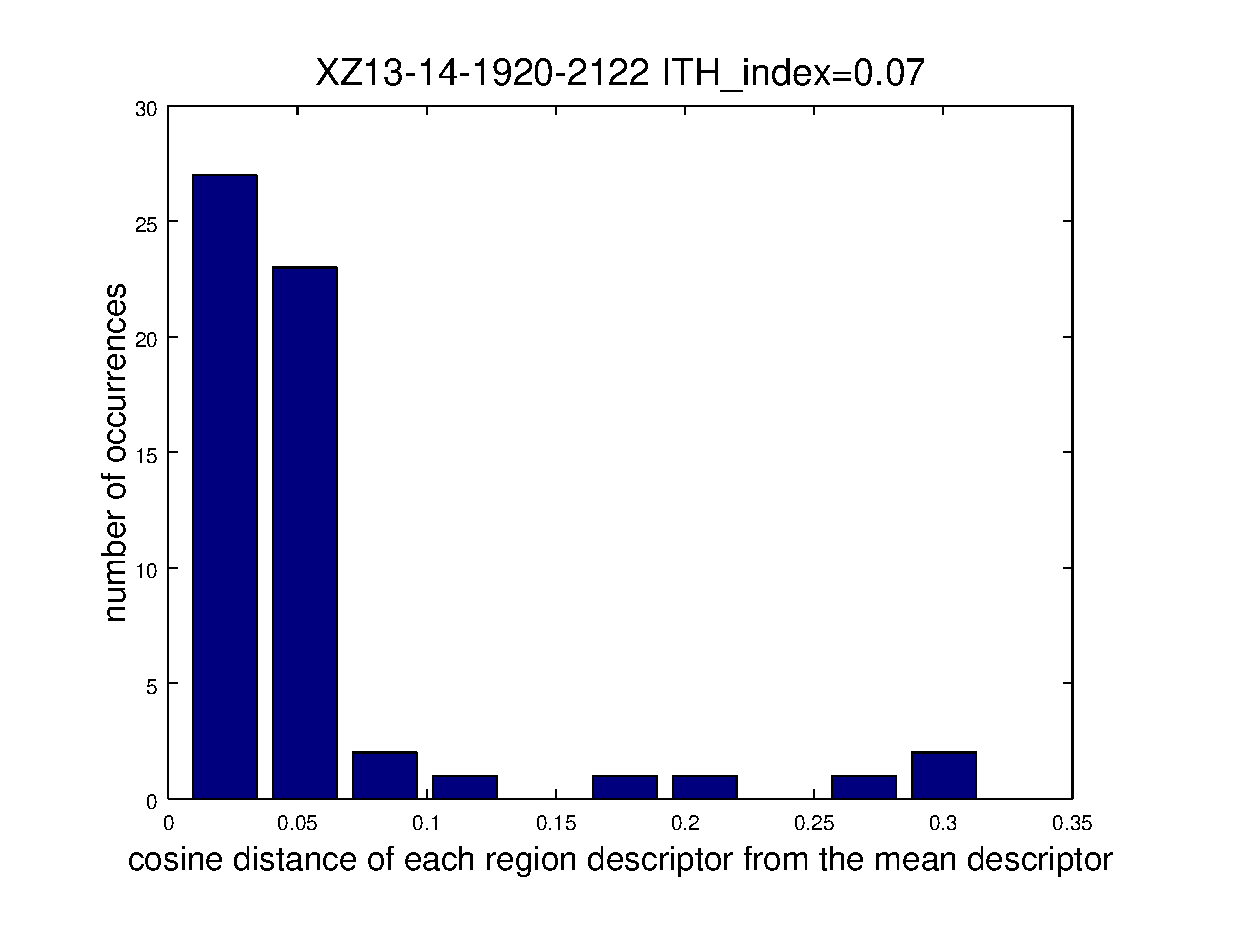
\includegraphics[scale=0.5]{histo_xz131419202122.eps}
\caption{Histogram of the cosine distances between mean and local descriptor. The ITH index is defined as the standard deviation of this distribution. Regions with less than 500 read counts have not been considered. The Shannon entropy is $2.58$ (using 50 bins for the histogram).}
\label{fig:histo_small}
\end{figure}

\begin{figure}[hbtp]
\centering
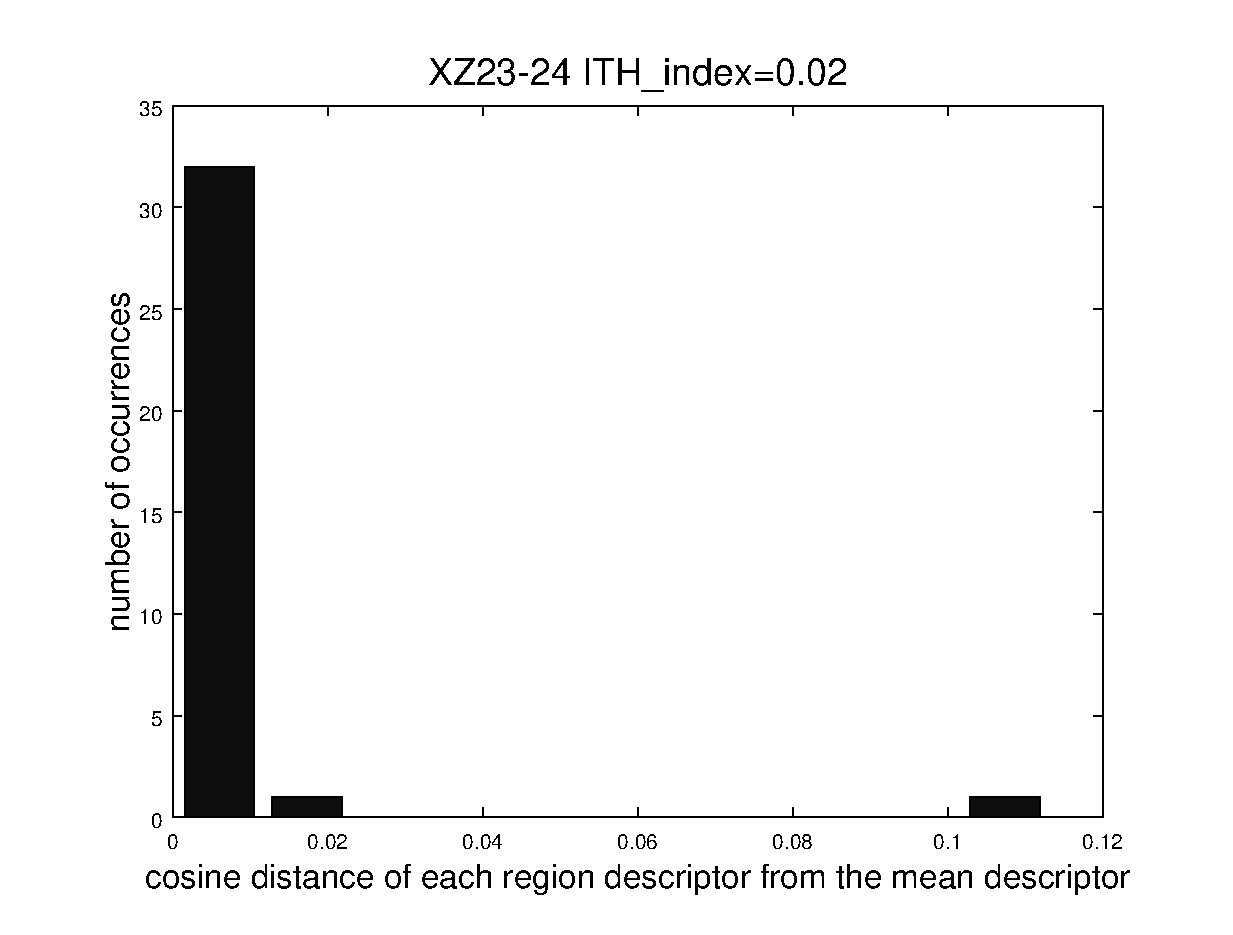
\includegraphics[scale=0.5]{histo_xz2324.eps}
\caption{Histogram of the cosine distances between mean and local descriptor. The ITH index is defined as the standard deviation of this distribution. Regions with less than 500 read counts have not been considered.}
\label{fig:histo_big}
\end{figure}

Fig.\ref{fig:histo_xz30} shows the distribution of distances from the mean of the regions coming from XZ30, which is related to a different breast cancer type and presents a higher ITH index compared to XZ23-24 (as expected from the sample composition of cells).

Instead of the standard deviation, one could also use the Shannon entropy to quantify ITH as expressed by the $d(\cdot;\cdot)$ distribution (see the captions of the figures to know the entropy values). 

\begin{figure}
\centering
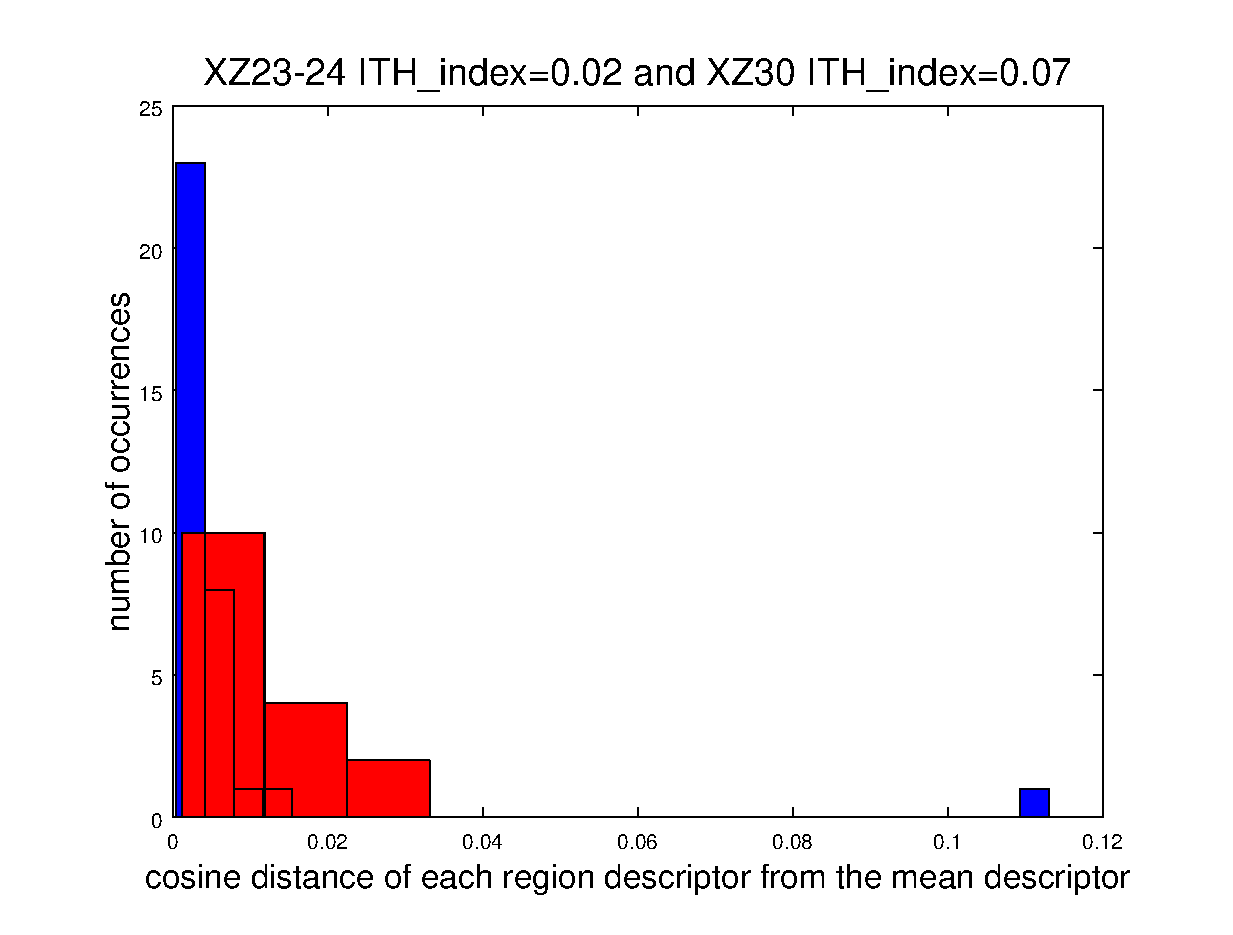
\includegraphics[scale=0.5]{histo_xz2324VSxz30.eps}
\caption{Histogram of the cosine distances between mean and local descriptor. The ITH index is defined as the standard deviation of this distributions. Regions with less than 500 read counts have not been considered. The red histogram (which covers part of the blue histogram) refers to XZ30, while the blue to XZ23-24. The Shannon entropy for XZ30 is $1.42$, for XZ23-24 is $1.30$ (using 50 bins for the histograms).}
\label{fig:histo_xz30}
\end{figure}

\section{TSS profile}
We consider the list of TSS for hg19, and we look at the number of unique reads 
falling into a given neighbourhood of each TSS. We then group the list of 
overlaps according to the gene name, and sort by the number of overlaps. This raw count could be biased by the number of cutsites in the interval 
around a TSS (the size of the interval will depend on details like having performed sonication or not). To take this into account, we evaluate for each TSS associated to a specific gene the number of cutsites around the TSS; in this way 
for each gene we know how many cutsites are supposed to be found close to it. The distribution of the frequency of cutsites is shown in Fig.\ref{fig:cutsite_distro}.

\begin{figure}
\centering
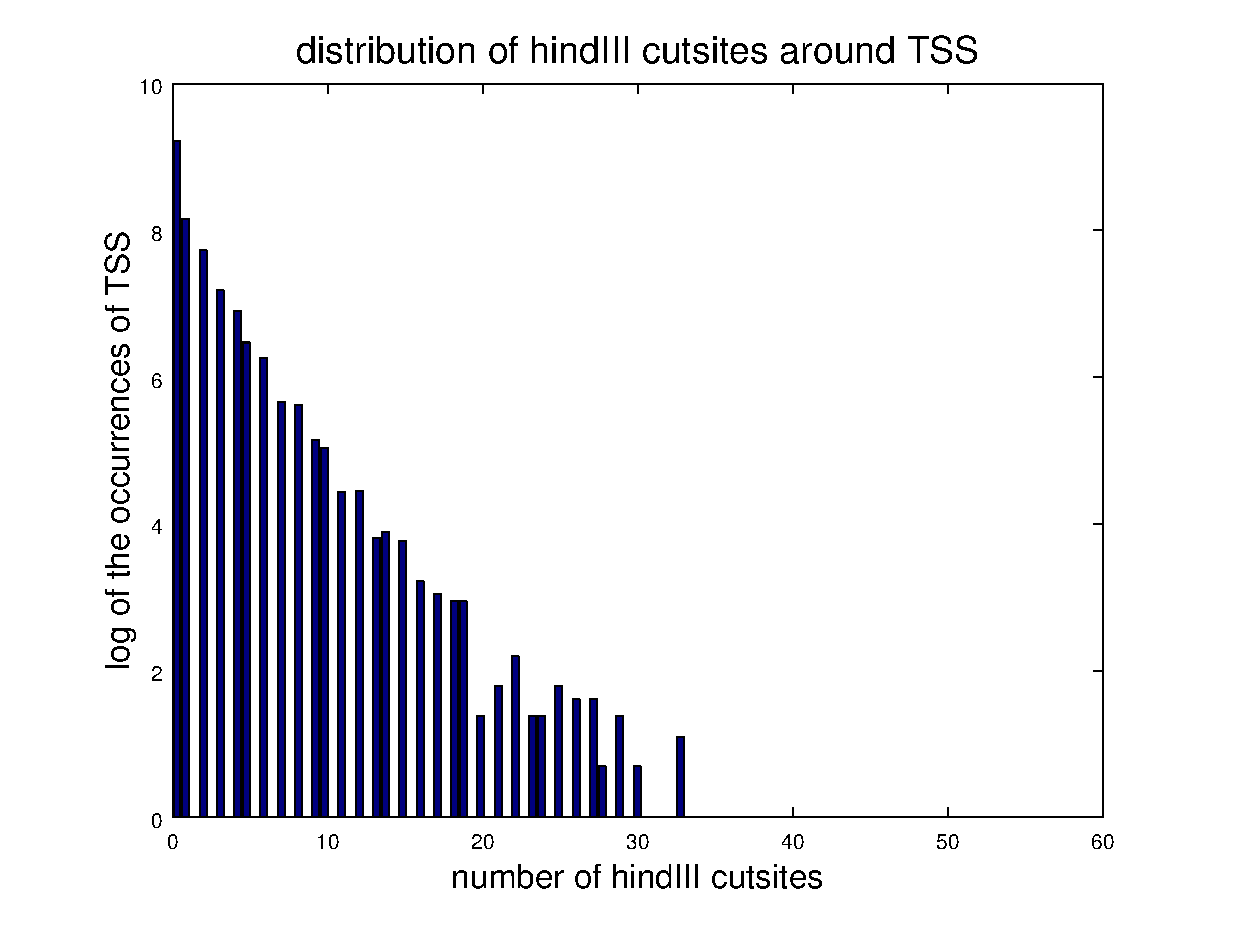
\includegraphics[scale=0.5]{distro_of_cutsites_around_TSS.eps}
\caption{Distribution of cutsites around a gene for a 1000bp window. Most of the genes have no cutsites around them, while few genes might have tens of cutsites around them. This motivates the need to normalize for the number of cutsites.}
\label{fig:cutsite_distro}
\end{figure}

\begin{figure}
\centering
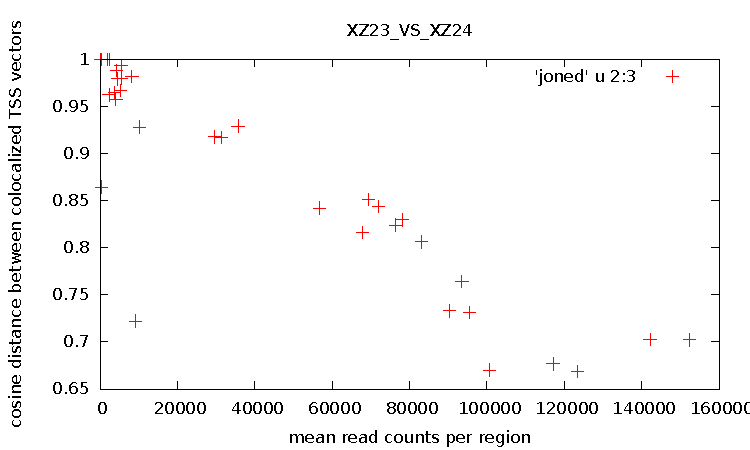
\includegraphics[scale=1]{distance_tss_noise.pdf}
\caption{Distance vs read counts for XZ23-24. This plot has to be compared with the analogous one for the DNA descriptor.}
\label{fig:noisetss}
\end{figure}

We now construct a TSS descriptor vector, as we have done for the DNA 
descriptor vector, and we repeat the previous DNA analysis (in terms of noise 
thresholding and ITH summary index) using the TSS descriptor. The TSS 
descriptor will list for each gene the number of reads and the number of 
cutsites found in a window around the gene's TSS locations, from which we can 
get the normalized read-count. Fig.\ref{fig:noisetss} show the behavior of the 
cosine distance for regions with different number of reads. A meaningful plot 
could be obtained only for XZ23-24, since for XZ19-20 and XZ21-22  the reads 
were too few to provide robust distances. The plot shows that the TSS descriptor is more affected by the noise than the corresponding DNA descriptor, which has to be expected since the latter has lower dimensionality (hence less features to use to be distinguished from another vector). This implies that we need to have more reads if we want to use this TSS vector description to compare datasets. Given this considerations I would not even try to derive an ITH index similar to the DNA descriptor, since we do not have datasets with enough reads. For completeness the following table provides some distances 
between TSS descriptors:

\begin{tabular}{|c|c|c|c|c|c|}
\hline 
• & xz23 & xz24 & xz30 & xz18+ & xz18- \\ 
\hline 
xz23 & 0 & 0.18 & 0.68 & 0.66 & 0.77 \\ 
\hline 
xz24 & • & 0 & 0.68 & 0.64 & 0.77 \\ 
\hline 
xz30 & • & • & 0 & 0.77 & 0.84 \\ 
\hline 
xz18+ & • & • & • & 0 & 0.72 \\ 
\hline 
xz18- & • & • & • & • & 0 \\ 
\hline 
\end{tabular} 
\newline

I would try to derive instead more general, less detailed, robust information 
from the TSS descriptors, such as: gene ranking and connections to known list of cancer related genes using for example the Human Protein Atlas database, PAM50, etc...
\subsection{PAM50}
Fig.\ref{fig:pam50_distro} show the distributions of normalized read-counts for all genes (excluding PAM50) and for PAM50 genes only. The idea is that PAM50 genes should have a larger weight towards the right side of the figures (higher expression). From the figures there is some weak evidence that this might be true.

\begin{figure}[htb]
\centering
  \begin{tabular}{@{}cccc@{}}
    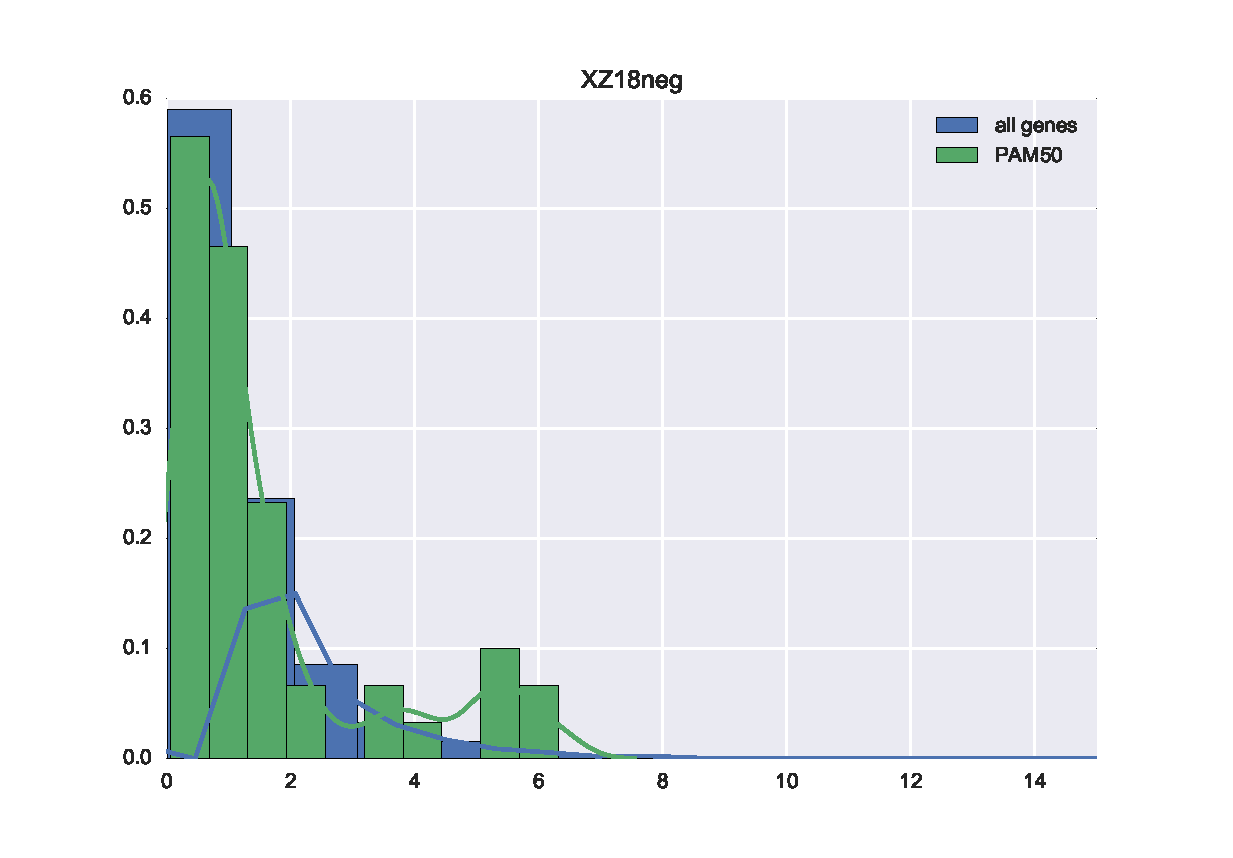
\includegraphics[width=.5\textwidth]{18neg.eps} &
    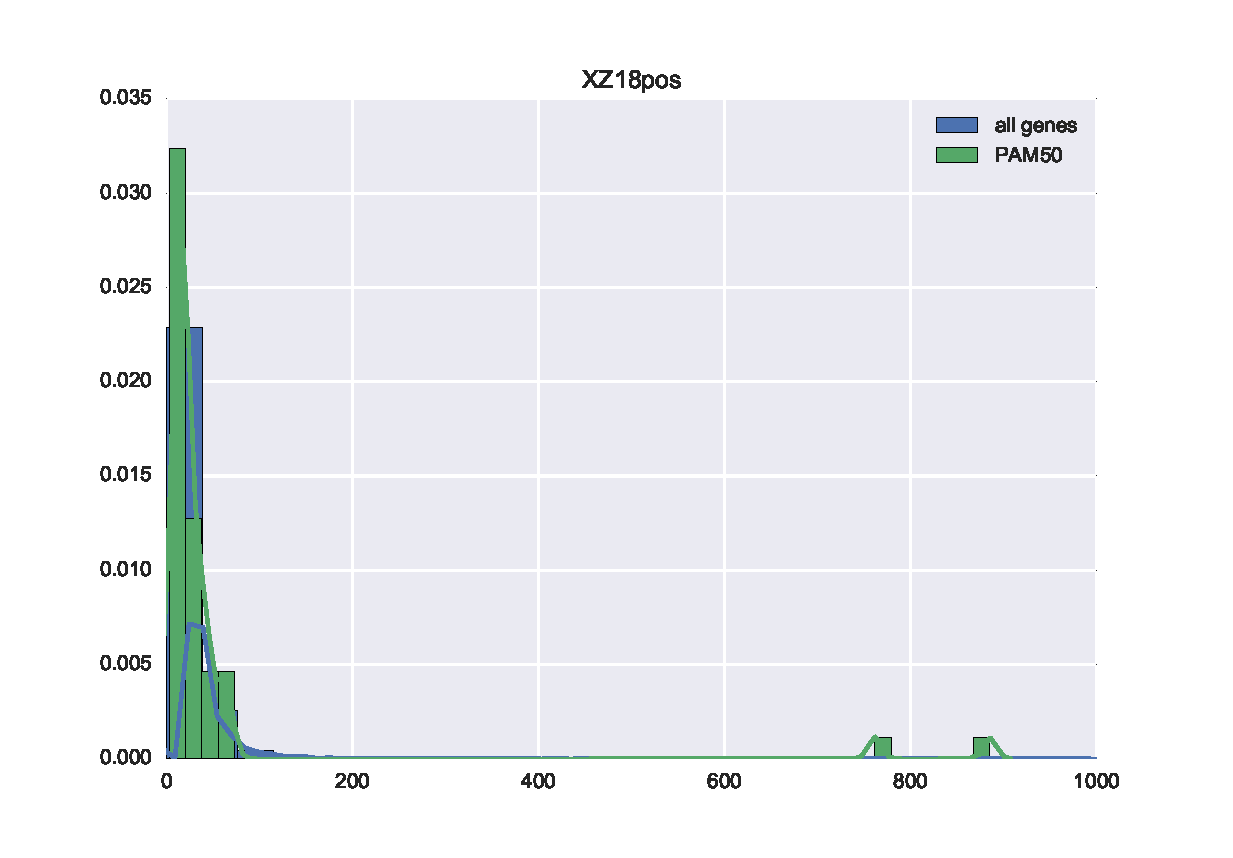
\includegraphics[width=.5\textwidth]{18pos.eps} \\
    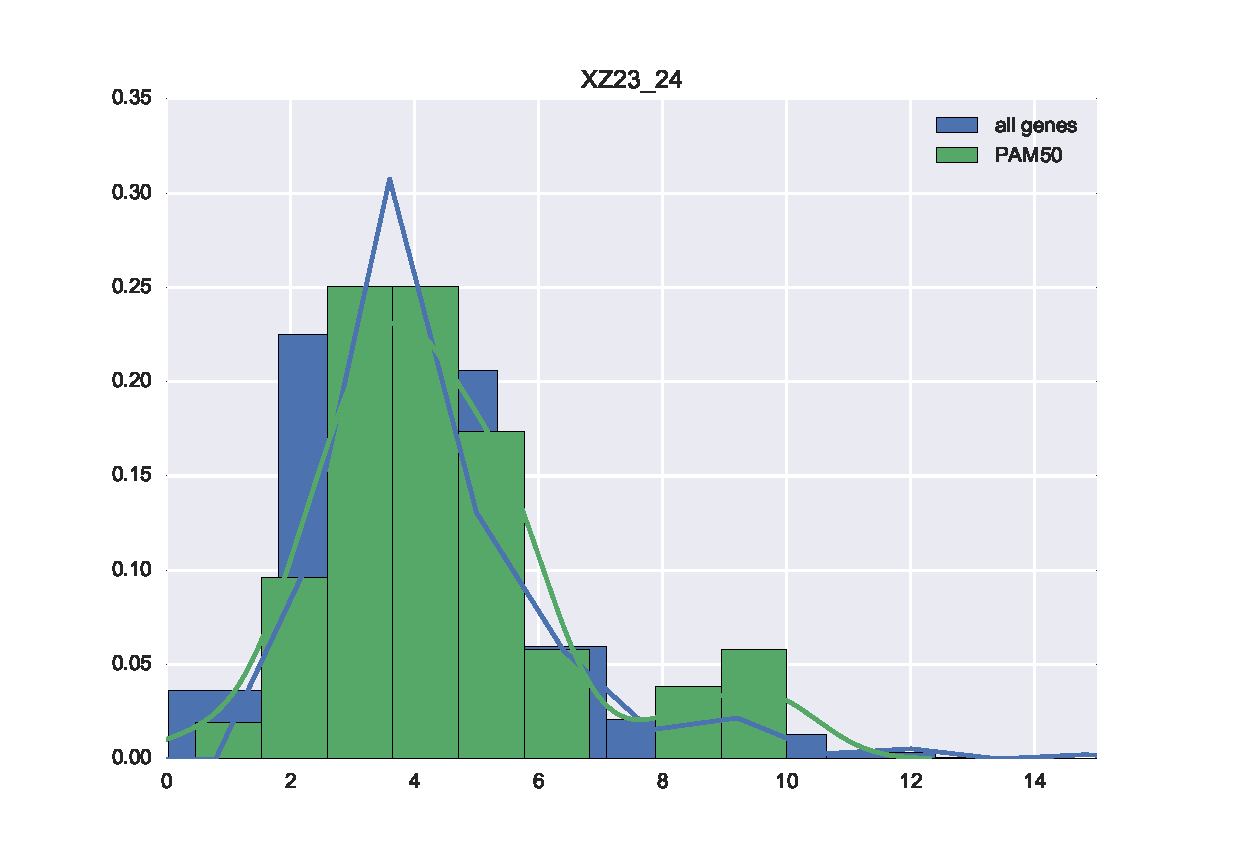
\includegraphics[width=.5\textwidth]{23_24.eps} &
    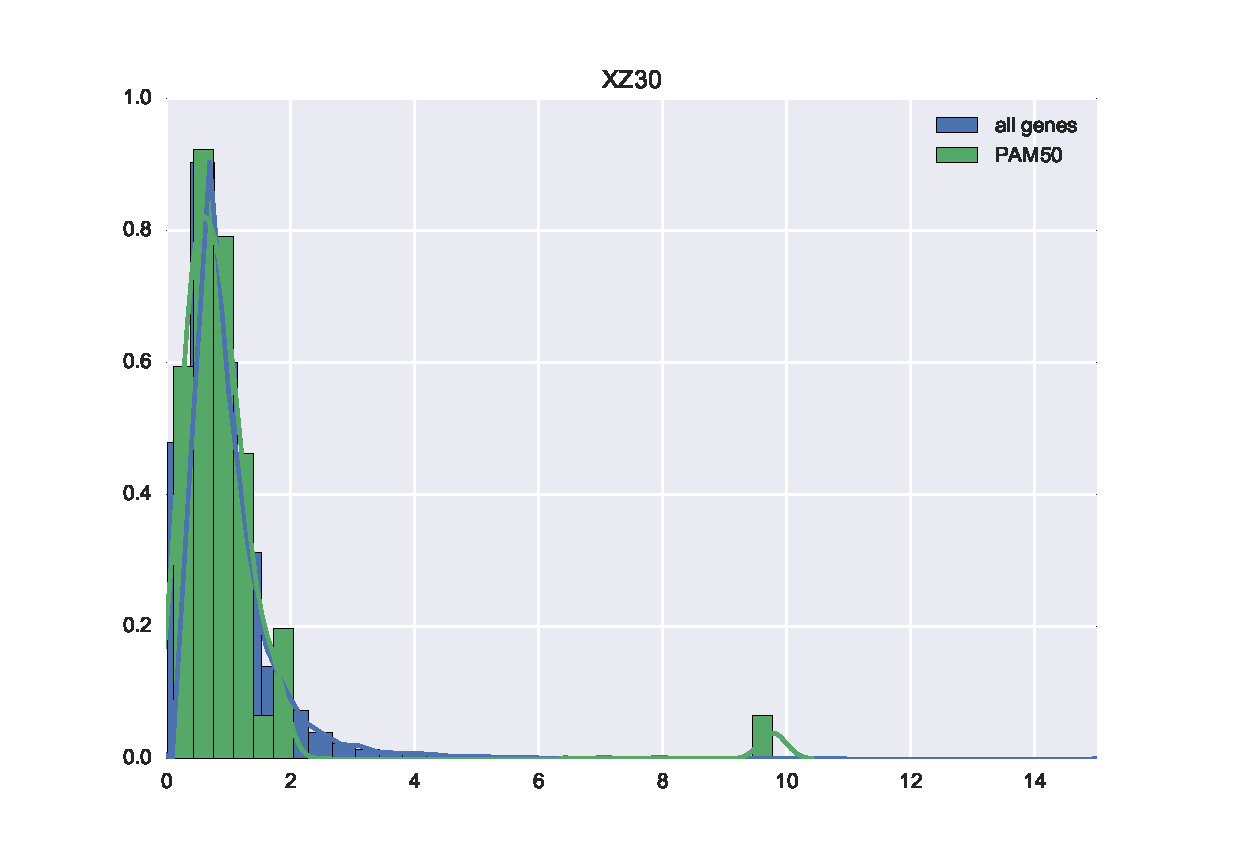
\includegraphics[width=.5\textwidth]{30.eps}   \\
  \end{tabular}
  \caption{Distributions of the read-counts for PAM50 genes and all other genes.}
  \label{fig:pam50_distro}
\end{figure}

This table shows the median normalized read-counts for PAM50 and all other genes:

\begin{tabular}{|c|c|c|}
\hline 
• & PAM50 & OTHERS \\ 
\hline 
xz30 & 0.79 & 0.75 \\ 
\hline 
xz23-24 & 4 & 3.7 \\ 
\hline 
xz18pos & 18.8 & 14.2 \\ 
\hline 
xz18neg & 0.85 & 0.82 \\ 
\hline 
\end{tabular} 

\section{Characterization of the errors in UMI}
Due to amplifications and sequencing the original UMI molecule might 
be subject to errors, and what we read in the fastq file is not what 
it is was supposed to be there at the beginning. 

To characterize these errors we consider NC85 (approx 33M reads output from sequencing), which does not contain 
any UMI and has a unique barcode which is supposed to be found before the 
cutsite. We select all the strings of 8bp which are found before a cutsite 
sequence at the beginning of the fastq file. Some of these strings will be 
subject to mismatch errors with respect to the original barcode: 

\begin{tabular}{|c|c|}
\hline 
errors & total \\ 
\hline 
6149605 & 27563642 \\ 
\hline 
\end{tabular} 

The number of mismatches found in all the error-strings is as follows:

\begin{tabular}{|c|c|}
\hline 
counts & number of MM \\ 
\hline 
4472524 & 1 \\ 
\hline 
1088701 & 2 \\ 
\hline 
410568 & 3 \\ 
\hline 
136272 & 4 \\ 
\hline 
34518 & 5 \\ 
\hline 
5972 & 6 \\ 
\hline 
847 & 7 \\ 
\hline 
203 & 8 \\ 
\hline 
\end{tabular}

as can be seen, grouping together co-localized UMI which differ by at most 2bp 
should take into account most of the mismatch-errors (90\% of the errors). 
Basically, using as an error model the prefix sequence UMI-barcode[1,0,0]-cutsite[1,0,0]-genomic we can recover 78\% of the potentially useful reads. While using UMI-barcode[1,0,0]-cutsite[2,0,0]-genomic we might be able to recover 80\% of the potentially useful reads. While using UMI-barcode[2,0,0]-cutsite[2,0,0]-genomic we might be able to recover 84\% of the potentially useful reads.

A similar analysis can be performed using XZ9 (approx 2M reads from sequencing), where we have many copies of a 
reference BARCODE(16)-CUTSITE(6)-Genomic. In total there are 1900898 reads, 
of which 1274568 have at most 1 mismatch in the cutsite location and are preceded by 16bp. Of these 1274568, 1273545 have at most 1 mismatch in the 8bp 
preceding the cutsite. Of the latter 1273545, 1272537 have at most 1 mismatch 
in the initial 8bp, and 1272876 have at most 2 mismatches in the initial 8bp. This experiment shows that 67\% of the reads show at most 1 mismatch in the cutsite location; 66.9\% show at most 1 mismatch in the cutsite location, and at most 1 mismatch in the barcode location. So, if we filter the initial fastq file for a prefix of the form UMI-barcode[1,0,0]-cutsite[1,0,0]-genomic we might loose approximately 30\% of the potentially useful reads. This percentage 
is not significantly lowered by allowing for more mismatches in the cutsite location or in the barcode location. 

Probably one should take into account insertions and deletions in order to use more reads downstream in the pipeline. The problem with these extensions of the error model is that the downstream read identification is made more ambiguous. Hence, for the moment, we prefer to stick with a more simple to recover but robust to false-positives error model: UMI-barcode[1,0,0]-cutsite[1,0,0]-genomic.

\section{Comparison between RNAseq and TISBA}
We have 4 datasets with RNA expression profiles (NC74-59-100-104) which 
can be compared respectively with the pool of SKBR3 cells TISBA-datasets, NC25, NC101 and NC 105, respectively. From the RNAseq data we select the list of top 25\% expressed genes, and the list of bottom \%25 expressed genes. For each of them we count the number of reads falling in a 5Kbp window around the associated TSS (in step of 500bp), and we normalize each read count by the number of cutsite in the same interval. The outcome of the analysis is shown in 
Fig.\ref{fig:rnaVSdna}.

\begin{figure}[htb]
\centering
  \begin{tabular}{@{}cccc@{}}
    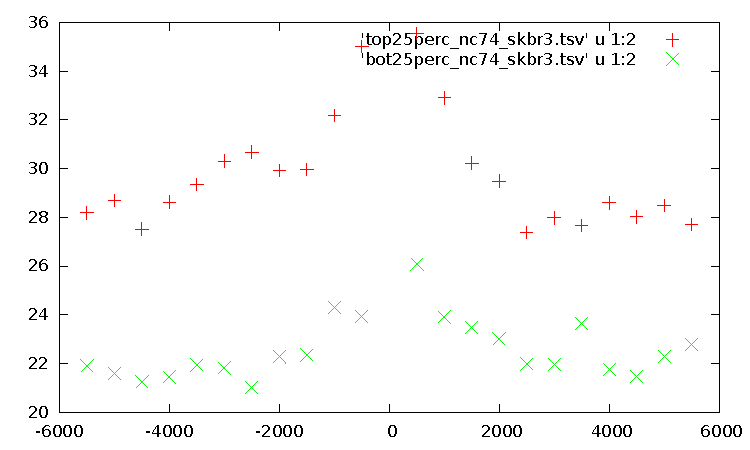
\includegraphics[width=.5\textwidth]{nc74_skbr3.pdf} &
    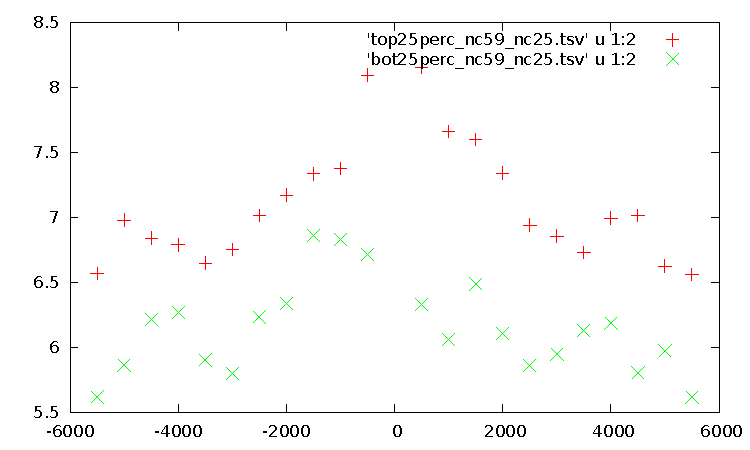
\includegraphics[width=.5\textwidth]{nc59_nc25.pdf} \\
    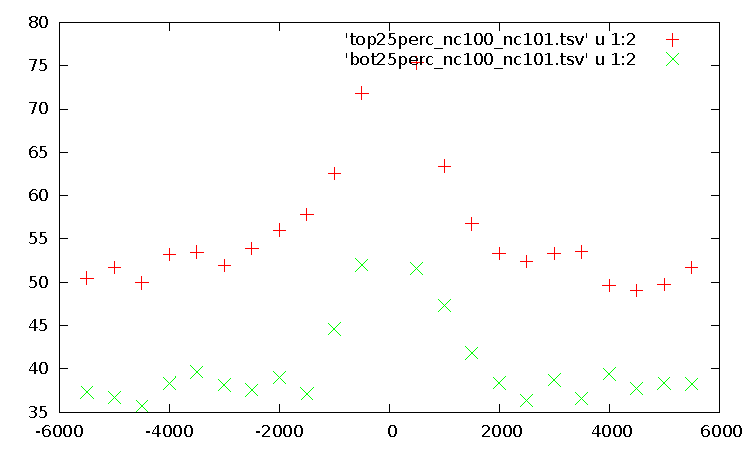
\includegraphics[width=.5\textwidth]{nc100_nc101.pdf} &
    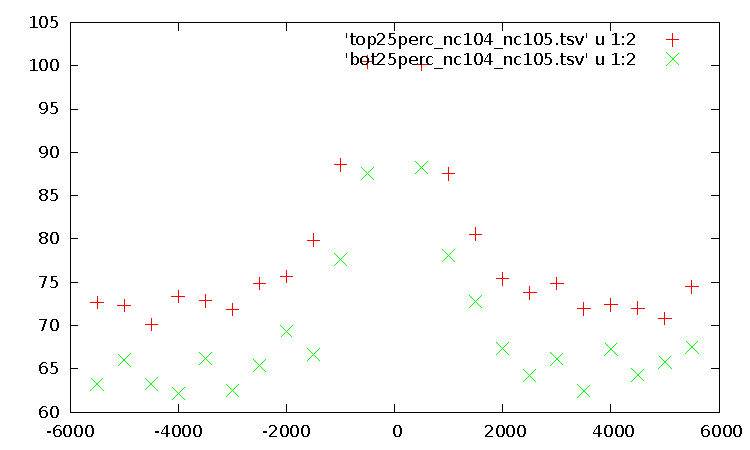
\includegraphics[width=.5\textwidth]{nc104_nc105.pdf}   \\
  \end{tabular}
  \caption{Average profiles around the TSSs of the top and bottom 25\% expressed genes, as measure by RNAseq. We plot the read counts in the vicinity of TSS normalized by the number of cutsites in the same interval, for each dataset.}
  \label{fig:rnaVSdna}
\end{figure}

As can be seen, for all datasets, the most expressed genes also provide a higher normalized read-count, supporting the correlation between accessibility (as measure by TBA) and expression (as measured by RNAseq).


\end{document}